\section{Proposed Approach}
\begin{frame}{Proposed Approach}
\framesubtitle{Evaluating VLMs for Pseudolabel Generation}
  \textbf{Approach:} Evaluate VLMs on generating \emph{accurate pseudolabels} for image classification datasets under various \emph{zero-shot} and \emph{few-shot} transfer conditions
  \vspace{0.3em}
    
  \begin{columns}[T]
    \column{0.55\textwidth}
      \centering \textbf{Key Research Aspects}
      \begin{enumerate}
        \item How does the \emph{number of examples} (few-shot vs. zero-shot) affect pseudolabel quality?
        \item What are the \emph{computational requirements} for practical application?
        \item How effective are the \emph{downstream models} trained on pseudolabels?
      \end{enumerate}

    \column{0.45\textwidth}
    \begin{figure}
      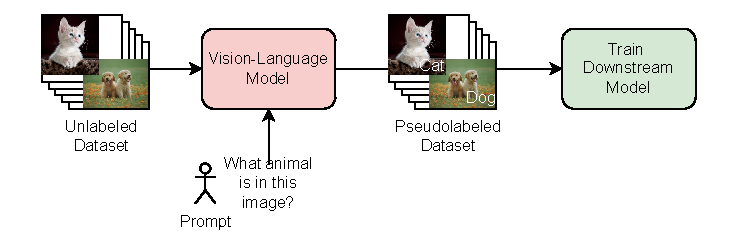
\includegraphics[width=\textwidth]{figures/vlm_transfer_downstream.pdf}
      \caption{\centering Using VLMs to generate pseudolabels for downstream model training}
    \end{figure}
  \end{columns}
\end{frame}
\note{
- Zero-shot means only describing the task in natural language; few-shot means providing examples \\
- We tested multiple prompting strategies to find the most effective approach \\
- We examined both common visual tasks (CIFAR-10) and specialized tasks (dermatology) to see if few-shot transfer is generalizable \\
- This design helps us understand when VLMs can be reliably transferred for automatic labeling \\
- For computational requirements, we measured inference time, memory usage, and scaling properties \\
- Downstream models were evaluated against models trained on ground truth labels \\
}


\section{Methodology}
\newcommand{\CifarDatasetSlide}{
\begin{columns}[T]
  \column{\customcolumnwidth}
    \textbf{Dataset Characteristics}
    \begin{itemize}
      \item 60,000 RGB images (32x32 pixels)
      \item 10 \emph{balanced} categories
      \item Standard split:
      \begin{itemize}
        \item 50,000 training
        \item 10,000 test (1,000/class)
      \end{itemize}
      % \item Categories:
      % \begin{itemize}
      %   \item Natural: birds, cats, deer, dogs, frogs, horses
      %   \item Artificial: airplanes, automobiles, ships, trucks
      % \end{itemize}
      \item \emph{Common} vision task
    \end{itemize}
  \column{\customcolumnwidth}
    \begin{figure}
    % CIFAR-10 examples figure
\begin{figure}[h]
  \begin{tabular}{ccccc}
    \begin{minipage}[b]{0.15\linewidth}
      
\includegraphics[width=\linewidth]{figures/cifar-images/airplane.png}
      \centering\scriptsize\texttt{airplane}
    \end{minipage} &
    \begin{minipage}[b]{0.15\linewidth}
      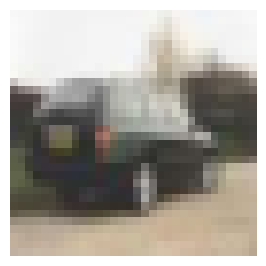
\includegraphics[width=\linewidth]{figures/cifar-images/automobile.png}
      \centering\scriptsize\texttt{auto}
    \end{minipage} &
    \begin{minipage}[b]{0.15\linewidth}
      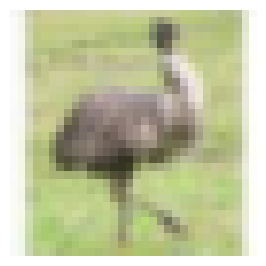
\includegraphics[width=\linewidth]{figures/cifar-images/bird.png}
      \centering\scriptsize\texttt{bird}
    \end{minipage} &
    \begin{minipage}[b]{0.15\linewidth}
      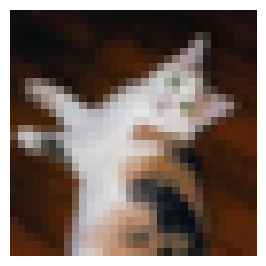
\includegraphics[width=\linewidth]{figures/cifar-images/cat.png}
      \centering\scriptsize\texttt{cat}
    \end{minipage} &
    \begin{minipage}[b]{0.15\linewidth}
      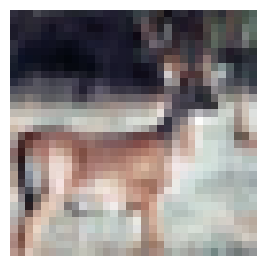
\includegraphics[width=\linewidth]{figures/cifar-images/deer.png}
      \centering\scriptsize\texttt{deer}
    \end{minipage} \\
    \begin{minipage}[b]{0.15\linewidth}
      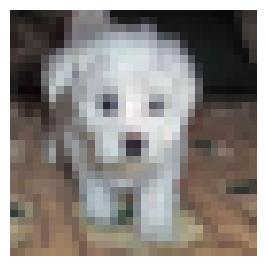
\includegraphics[width=\linewidth]{figures/cifar-images/dog.png}
      \centering\scriptsize\texttt{dog}
    \end{minipage} &
    \begin{minipage}[b]{0.15\linewidth}
      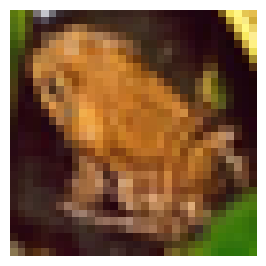
\includegraphics[width=\linewidth]{figures/cifar-images/frog.png}
      \centering\scriptsize\texttt{frog}
    \end{minipage} &
    \begin{minipage}[b]{0.15\linewidth}
      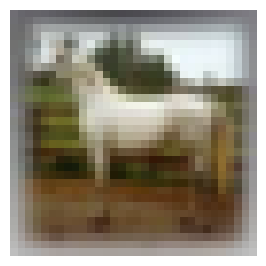
\includegraphics[width=\linewidth]{figures/cifar-images/horse.png}
      \centering\scriptsize\texttt{horse}
    \end{minipage} &
    \begin{minipage}[b]{0.15\linewidth}
      
\includegraphics[width=\linewidth]{figures/cifar-images/ship.png}
      \centering\scriptsize\texttt{ship}
    \end{minipage} &
    \begin{minipage}[b]{0.15\linewidth}
      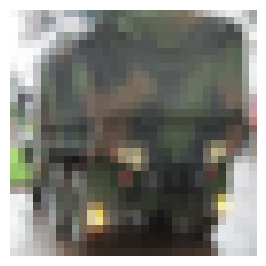
\includegraphics[width=\linewidth]{figures/cifar-images/truck.png}
      \centering\scriptsize\texttt{truck}
    \end{minipage}
  \end{tabular} 
\end{figure}
    \caption{Example images from CIFAR-10~\footfullciteieee{Krizhevsky2009}}
    \end{figure}
\end{columns}
}
\subsection{Datasets}
\begin{frame}{Datasets Used}
  \framesubtitle{CIFAR-10 Dataset}
  \vspace{-1em}
  \CifarDatasetSlide
\end{frame}
\note{

}

\newcommand{\DermPtDatasetSlide}[1]{
\begin{columns}[T]
  \column{\customcolumnwidth}
    \textbf{Dataset Characteristics}
    \vspace{-0.4em}
    \begin{itemize}
      \item 1,011 dermatological cases for melanoma diagnosis (as well as other skin conditions)
      \item Multiple image modalities:
        \begin{itemize}
          \item Dermoscopic (standardized)
          \item Clinical (varying conditions)
        \end{itemize}
      % \item Dataset split (diagnoses and features not uniform):
      %   \begin{itemize}
      %     \item 413 training cases
      %     \item 203 validation cases
      %     \item 395 test cases
      %   \end{itemize}
      \item Diagnoses and features are not uniformly distributed
      \item Task-specific dataset -- likely not present in VLM pre-training data
    \end{itemize}
  \column{\customcolumnwidth}
    \vspace{-0.5em}
    #1
\end{columns}
}

\newcommand{\DermPtFigureOne}{
  \begin{figure}[h]
    \centering
    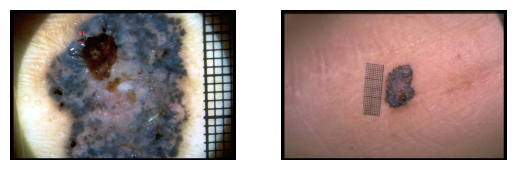
\includegraphics[width=0.9\linewidth]{figures/derm7pt-images/derm_01.png}
    \vspace{0.25em}
    \raggedright
    \scriptsize\texttt{diagnosis}: basal cell carcinoma\\
    \scriptsize\texttt{pigment\_network}: absent\\
    \scriptsize\texttt{streaks}: absent\\
    \scriptsize\texttt{pigmentation}: absent\\
    \scriptsize\texttt{regression\_structures}: blue areas\\
    \scriptsize\texttt{dots\_and\_globules}: irregular\\
    \scriptsize\texttt{blue\_whitish\_veil}: present\\
    \scriptsize\texttt{vascular\_structures}: within regression\\
    \vspace{0.25em}
    \scriptsize\texttt{seven\_point\_score}: 4\\
    \scriptsize\texttt{level\_of\_diagnostic\_difficulty}: low
    \caption{\centering An example case from Derm7Pt}
  \end{figure}
}

\newcommand{\DermPtFigureTwo}{
  \begin{figure}[h]
    \centering
    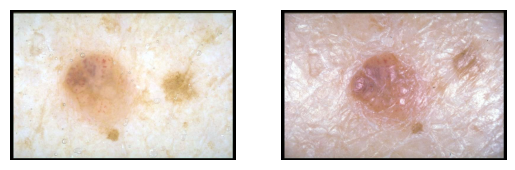
\includegraphics[width=0.9\linewidth]{figures/derm7pt-images/derm_02.png}
    \vspace{0.25em}
    \raggedright
    \scriptsize\texttt{diagnosis}: melanoma metastasis\\
    \scriptsize\texttt{pigment\_network}: absent\\
    \scriptsize\texttt{streaks}: absent\\
    \scriptsize\texttt{pigmentation}: diffuse irregular\\
    \scriptsize\texttt{regression\_structures}: absent\\
    \scriptsize\texttt{dots\_and\_globules}: regular\\
    \scriptsize\texttt{blue\_whitish\_veil}: absent\\
    \scriptsize\texttt{vascular\_structures}: hairpin\\
    \vspace{0.25em}
    \scriptsize\texttt{seven\_point\_score}: 1\\
    \scriptsize\texttt{level\_of\_diagnostic\_difficulty}: high
    \caption{\centering A particularly challenging example case from Derm7Pt}
  \end{figure}
}

\begin{frame}{Datasets Used}
  \framesubtitle{Seven-Point Checklist Dermatology Dataset (Derm7Pt)}
  \vspace{-1em}
  \DermPtDatasetSlide{\DermPtFigureOne}
\end{frame}
\note{
- The Derm7Pt dataset is a collection of dermatological images and annotations for melanoma diagnosis, as well as other skin conditions such as seborrheic keratosis, basal cell carcinoma, types of nevi, and more \\
- A seven point score of greater than or equal to 3 is to be referred for specialist analysis for melanoma \\
- The authors provide a python library as an interface to the dataset, and perform grouping of rare cases as well as the grouping of fine-grained categorization into more coarse categories \\
- In the authors' paper, it is shown that incorporating clinical images as input to their CNN model improves performance \\
}


\subsection{Models Chosen}
\begin{frame}{Models Chosen}
\framesubtitle{Which models did we evaluate?}
  \vspace{-1em}
  \begin{columns}[T]
    \column{\customcolumnwidth}
    \begin{itemize}
      \item \textbf{InternVL2-8B:} 8B parameters, 8k context window
      \item \textbf{MiniCPM-V-2.6:} 8B parameters, \emph{image token compression} with \emph{perceiver-resampler} architecture
      \item \textbf{Pixtral 12B:} 12B parameters, 128K context window, \emph{handles images natively}
    \end{itemize}
    \column{\customcolumnwidth}
    \begin{itemize}
      \item \textbf{Phi-3.5-Vision-Instruct:} 4B parameters, 128K context window, designed for constrained environments
      \item \textbf{Bio-Medical-MultiModal-Llama-3-8B-V1:} 8B parameters, \emph{fine-tuned} multimodal adaptation of Llama-3.1-8B-Instruct for \emph{biomedical} tasks
    \end{itemize}
  \end{columns}
  \textbf{Notes:}
  \begin{itemize}
    \setlength{\itemsep}{0em}
    \item All models use towered architectures, integrating visual encoders with language models, with \emph{integrated image} tiling, \emph{processing} methods (except for Pixtral)
    \item Models chosen for claimed ability in processing \emph{interleaved} image-text inputs
  \end{itemize}
\end{frame}
\note{
- InternVL2-8B and MiniCPM-V-2.6 models integrate visual and language processing components \\
- Phi-3.5-vision-instruct and Pixtral 12B models are designed for long-context multimodal processing \\
- Bio-Medical-MultiModal-Llama-3-8B-V1 is specialized for biomedical tasks \\
- Models selected for their ability to handle multi-image, multi-turn multimodal conversations, or in other words, interleaved text and image inputs \\
- Notably, all models use their own integrated image tiling and processing methods, except for the Pixtral 12B model, which processes images natively at their full resolution without tiling
}


\subsection{Experimental Design}
\begin{frame}{Experimental Design}
\framesubtitle{How did we evaluate VLMs?}
  \vspace{-1em}
  \begin{itemize}
    \item \textbf{Zero-Shot Transfer:}
    \begin{itemize}
      \item Evaluated ability to perform tasks \emph{without prior examples}
      \item Used basic and enhanced prompts with task-specific information and chain-of-thought reasoning
    \end{itemize}
    \item \textbf{Few-Shot Transfer:}
    \begin{itemize}
      \item Assessed effects of \emph{providing examples} on model performance, resource usage
      \item Explored pure few-shot experiments and combinations with prompting
    \end{itemize}
    \item \textbf{Downstream Model Training:}
    \begin{itemize}
      \item Evaluated \emph{knowledge transfer} by training downstream models from pseudolabels
      \item Analyzed effects of transfer methods on downstream model performance
    \end{itemize}
  \end{itemize}
\end{frame}
\note{
- Zero-shot learning assessed through basic and enhanced prompts \\
- Few-shot learning explored with varying examples and combinations \\
- Downstream training focused on pseudolabel effectiveness \\
- Comprehensive evaluation framework used to assess VLM capabilities \\
}


% \subsection{Prompting and VLM Inputs}
\begin{frame}{Prompting and VLM Inputs}
\framesubtitle{How did we prompt the VLM?}
  \vspace{-1em}
  A \emph{Prompting Framework} was developed, that:
  \begin{itemize}
    \item Employed a consistent \emph{chat-based} interaction format for fair comparison
    \item Isolated effects of different prompting components (zero-shot, few-shot, reasoning) with a \emph{modular} prompt structure
    \item \emph{Minimized biases} through systematic, deterministic and reproducible \emph{randomization} of class lists and example ordering
  \end{itemize}
\end{frame}
\note{
- Prompting strategy focused on fair comparison and isolating effects of different components \\
- Chat-based format maintained consistency across experiments \\
- Standardized preprocessing and prompt templates ensured reproducibility \\
- Deterministic random seeds used for example selection and class list shuffling \\
- Core structure included base prompt, example integration, and test instance presentation \\
}


\begin{frame}{Prompting and VLM Inputs}
\framesubtitle{How did we prompt the VLM?}
  \vspace{-1em}
  \begin{columns}[T]
    \column{\customcolumnwidth}
    \textbf{Core Structure of the Prompt:}
    \begin{itemize}
      \item \textbf{Base Prompt Structure:} \emph{Guides models} with task definition and output format
      \item \textbf{Example Integration:} Alternating user-assistant message pairs for \emph{few-shot examples}
      \item \textbf{Test Instance Presentation:} Test image presented for classification in \emph{final turn}
    \end{itemize}
    \column{\customcolumnwidth}
    \vspace{-4em}
    \begin{figure}
      \centering
      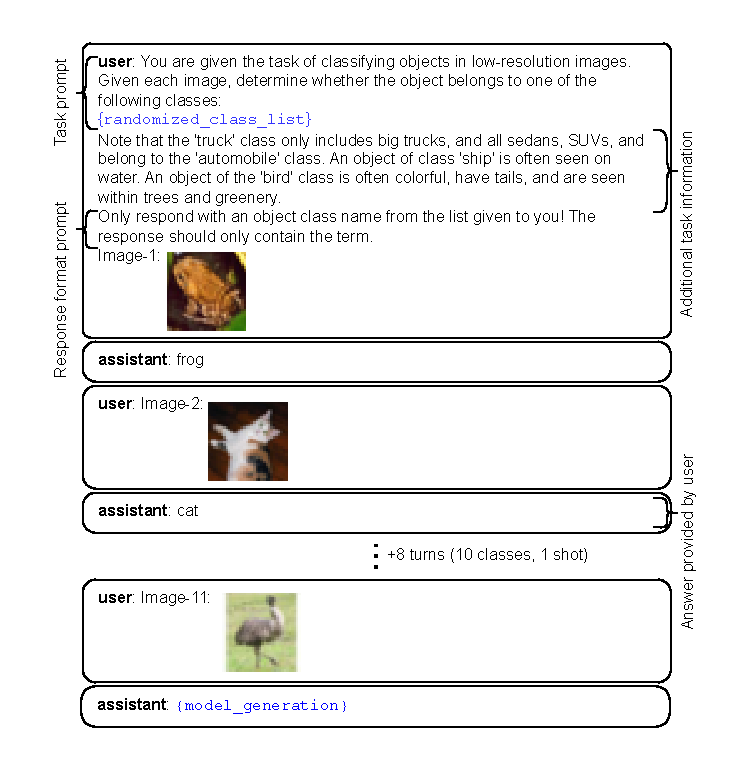
\includegraphics[width=1.12\linewidth]{figures/prompt_building.pdf}
      \vspace{-2.4em}
      \caption{Visualization of the prompt building process}
    \end{figure}
  \end{columns}
\end{frame}
\note{
- The example shown is for the CIFAR-10 dataset. A similar process is used for the Derm7Pt dataset, but with category-specific prompts for each category and the optional addition of clinical images \\
- Base prompt structure guides models with task definition, class list, reasoning requirements, and output format
- Alternating user-assistant message pairs for few-shot examples -- answers are provided by user
- Final turn presents test image for classification -- answer is provided by model
}